\chapter{Experimental Approach}

The experiments presented here were conducted in Prague and Lancaster independently. There are many experimental ways how to launch the production of quantum turbulence: by an oscillating objects (wires, the tuning forks, oscillating discs, etc.) or by a \textit{coflow} and \textit{counterflow} techniques.

In our investigation, we used the tuning fork oscillator, driven by alternating source Agilent A33220 and measured by SR830 amplifying lock-in. We measured both the in-phase and anti-phase componentes of signals. Results from other oscillators' measurements are included in this Thesis, however, not performed by the Thesis author.

\section{Apparatus}

All the measurements were performed in a helium cryostat (\textbf{Figure \ref{cryostat}}), cooled down to the desired temperatures using a rotary and Roots pump, and stabilized (with errors of a few mK) either manually or using the temperature controller. The working temperatures are from a wide range from a little above $T_{\lambda}$ to the lowest (experimentally) possible one $T_{min} \approx 1.3\unit{K}$. We also added series of measuremens from area far above $T_{\lambda}$, when $T = 3000\unit{K}$ to be confident about the hydrodynamical regime. The range $(1.3\unit{K} - 2.17\unit{K})$ allows access to most of the two-fluid regime.

\begin{figure}[h]
	\centering
	\includegraphics[width=0.8\textwidth]{graphics/exp/apparatus}
	\caption{A photograph of the experimental setup. From left: source generators, lock-in, cryostat, pipe system for emerging gas, Roots pump. Source: \cite{bakalaris}}
	\label{cryostat}
\end{figure}

\newpage

Measurements at temperatures $T < 0.6\unit{K}$ temperatures in the ballistic regime were performed on a Leiden Cryogenics MNK126-400 dilution refrigerator with a base temperature below $10 \unit{mK}$. These sub-Kelvin measurement description is not included in this Thesis. However, refrigerator results are used in \textbf{Results} part to demonstrate the uniform scaling theory.

Resonator was attached at the bottom (\textbf{Figure \ref{resonator}}) of the \textit{insert} - a large metalllic construction holding all mezsuring micro-devices. Insert serves as an vertical injection to the cryostat, filled continuously with helium from above. Therefore, resonator was place at the bottom, to ensure that it is submerged as long as possible.

\begin{figure}[h]
	\centering
	\includegraphics[width=0.8\textwidth]{graphics/exp/chamber}
	\caption{A photograph of the resonator attached at the bottom of metallic insert. Source: \cite{bakalaris}}
	\label{resonator}
\end{figure}

To obtain the best results at low temperatures both in vacuum and superfluid helium, the Prague cell containing the oscillators was flushed repeatedly with dry nitrogen gas prior to cooling. Each time it was pumped down below $\approx 10^{-5}\unit{mbar}$ using a turbomolecular pump.

After the last evacuation (to $\approx 10^{-6}\unit{mbar}$), the direct connection was closed off. With reasonable confidence that no helium ices could form on the resonators at low temperature, we strated ti fill the cell with pure superfluid 4-Helium. At this point, all calibrations of thermometers and resonators were made.


\newpage

\section{Resonators}

In this part we briefly describe the principles of small oscillating resonators used in Helium-II experiments.

\subsection*{Vibrating Wire}

Vibrating wire resonator consists of a semi-circular loop of wire inserted to a vertical magnetic field $\vec{B}$, as shown in \textbf{Figure \ref{wire}}. As we turn on the alternating current flux $\vec{j} \propto e^{i\omega t}$ inside the wire, these currents forces the wire to oscillate due to Lorentz force $\vec{F}_L \propto \vec{j} \times \vec{B} $. As the wire is moves through the field, the Faraday voltage is induced of magnitude \cite{universal_scaling}:

\begin{equation}
V = - \frac{\text{d} (\vec{B} \dotprod \vec{S})}{\text{d} t}
\sim \frac{\pi}{4} BDU\,,
\end{equation}

where $\vec{S}$ is the area vector, enclosed by the wire loop and $D$ is the distance between wire's legs. Experimentally used magnetic fields were in range $(170 \pm 10) \unit{mT}$.

\begin{figure}[h]
	\centering
	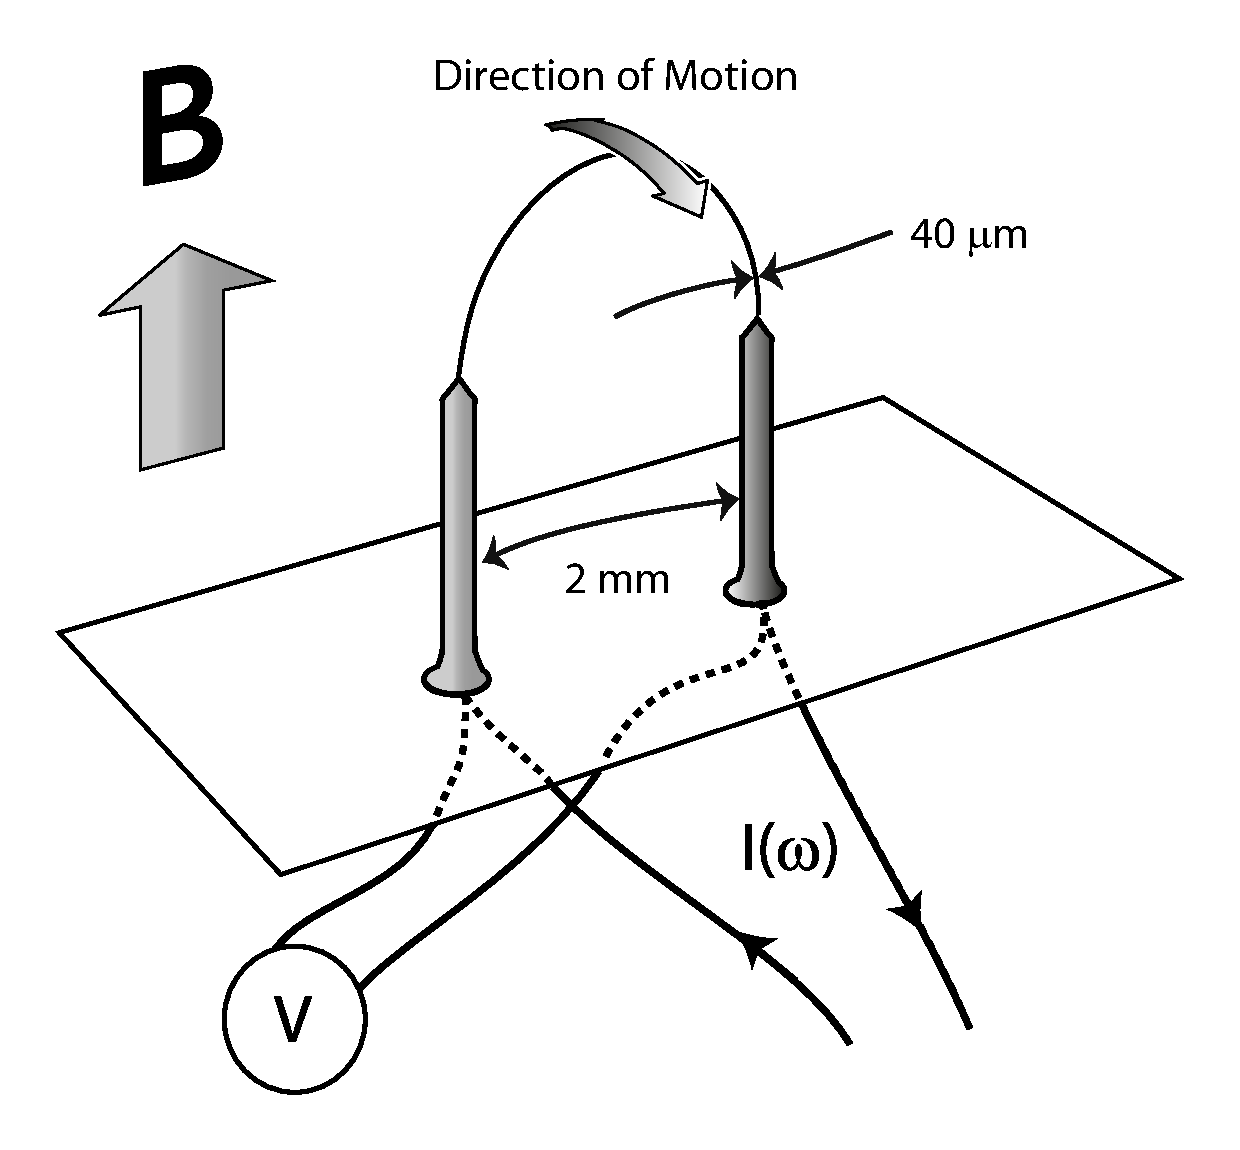
\includegraphics[width=0.5\textwidth]{graphics/exp/wire}
	\caption{Schematic diagram of the vibrating wire resonator. Source: \cite{universal_scaling}}
	\label{wire}
\end{figure}

\newpage

\subsection*{Tuning Fork}

Quartz tuning forks (TF) are commercial piezoelectric oscillators with a well-calibrated resonant frequency. They are usually used as frequency standards in watches or as force sensors in microscopes. Also, TFs have started to be widely used in cryogenic Helium II experiments.

In our experimental work, we used the fork of following dimensions: prongs length $ \mathcal{L} = 3.50\unit{mm} $, prongs width (perpendicular to the fork plane) $ \mathcal{W}=75 \mu\unit{m} $, thickness $ \mathcal{T}=90\mu\text{m} $ prongs interdistance $ \mathcal{D}=90\mu\text{m} $.\\
A sketch of the fork architecture is depicted in \textbf{Figure \ref{fork}}:

\begin{figure}[h]
	\centering
	\includegraphics[width=0.25\textwidth]{graphics/exp/quartz}
	\caption{Schematic diagram of the quartz tuning fork. Source: \cite{bakalaris}}
	\label{fork}
\end{figure}

There are several achievable resonant modes at which the fork can oscillate. We chose to work with the \textit{fundamental} one at $f_0 = 6.7 \unit{kHz}$ and with the first \textit{overtone} one at $f_1 = 41 \unit{kHz}$.\\
The fork is driven by applying an alternate voltage $V(t) \propto e^{i\omega t}$ from a generator to the metalic plates (deposited on fork surface). The piezoelectric effect causes a tension resulting in a force, which is proportional to the applied voltage. In fundamental mode, the fork exhibits an anti-phase oscillating motion of its prongs with a single node. In case of overtone, there would be just two nodes. The fork's flex induces a piezoelectric current $I(t)$ about which is shown its proportionality to the velocity $U(t)$.

\newpage

The conversion relations between applied $V(t)$, measured $I(t)$ and mechanical properties $F(t)$, $U(t)$ are given \cite{fork} as:

\begin{equation}
F(t) = \frac{1}{2} a_{rmf} V(t)\,,
\hspace{1cm}
U(t) = \frac{I(t)}{a_{rmf}}\,,
\end{equation}

where $a_{rmf}$ is the so-called \textit{fork constant}. This constant can be derived from a fork's geometry, material and an oscillation mode. Usually the formula for this constant is given by a deflection measurement:

\begin{equation}
a_{rmf} = \sqrt{4\pi m_{eff} \Delta f \frac{I}{V}}\,,
\end{equation}

where $m_{eff} = TWL\rho_q /4$ ($\rho_q$ as the quartz density) is the fork's effective mass and $\Delta f$ is the measured peak width from the fequency-sweep deflection measurement. In our case we used fork with the effective mass and fork constants for fundamental and overtone mode of following values:

\begin{equation}
m_{eff} = 1.52 \times 10^{-2} \mu\unit{g}\,,
\hspace{1cm}
a_0 = 0.3 \mu\unit{Cm}^{-1}\,,
\hspace{1cm}
a_1 = 1.41 \mu\unit{Cm}^{-1}
\end{equation}

The measurement scheme for the Prague experiment with tuning fork is shown in \textbf{Figure \ref{setup}}. The arrangement of other experiments in Lancaster were slightly more complex, but similar.

\begin{figure}[h]
	\centering
	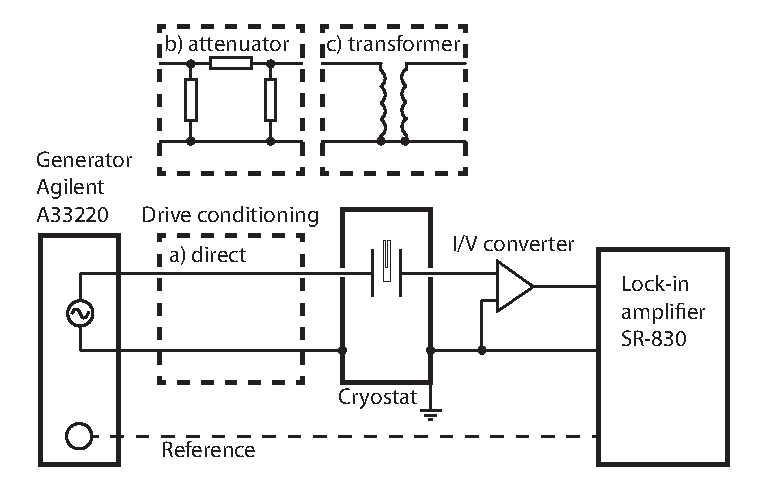
\includegraphics[width=0.6\textwidth]{graphics/exp/fork_setup}
	\caption{Diagram of the measurement scheme used in Prague. To achieve the full range of velocities, the applied voltage was either (a) directly fed to the tuning fork, (b) attenuated by one or more inline attenuators, or (c) amplified by a transformer. The transformer’s output was constantly monitored. Source: \cite{multiple-vels}}
	\label{setup}
\end{figure}

\newpage

\subsection*{Oscillating Disc}

The torsional oscillator consists of a $50 \mu\unit{m}$ wire  with a glass disc fixed to
the wire at its midpoint. The disc is $1\unit{mm}$ thick with a diameter of $40\unit{mm}$. A schematic picture is showed in \textbf{Figure \ref{disc}}.\\
Sixteen black marks around the circumference of the disc are used to determine the deflection and angular velocity of the disc from recorded video sequences.

\begin{figure}[h]
	\centering
	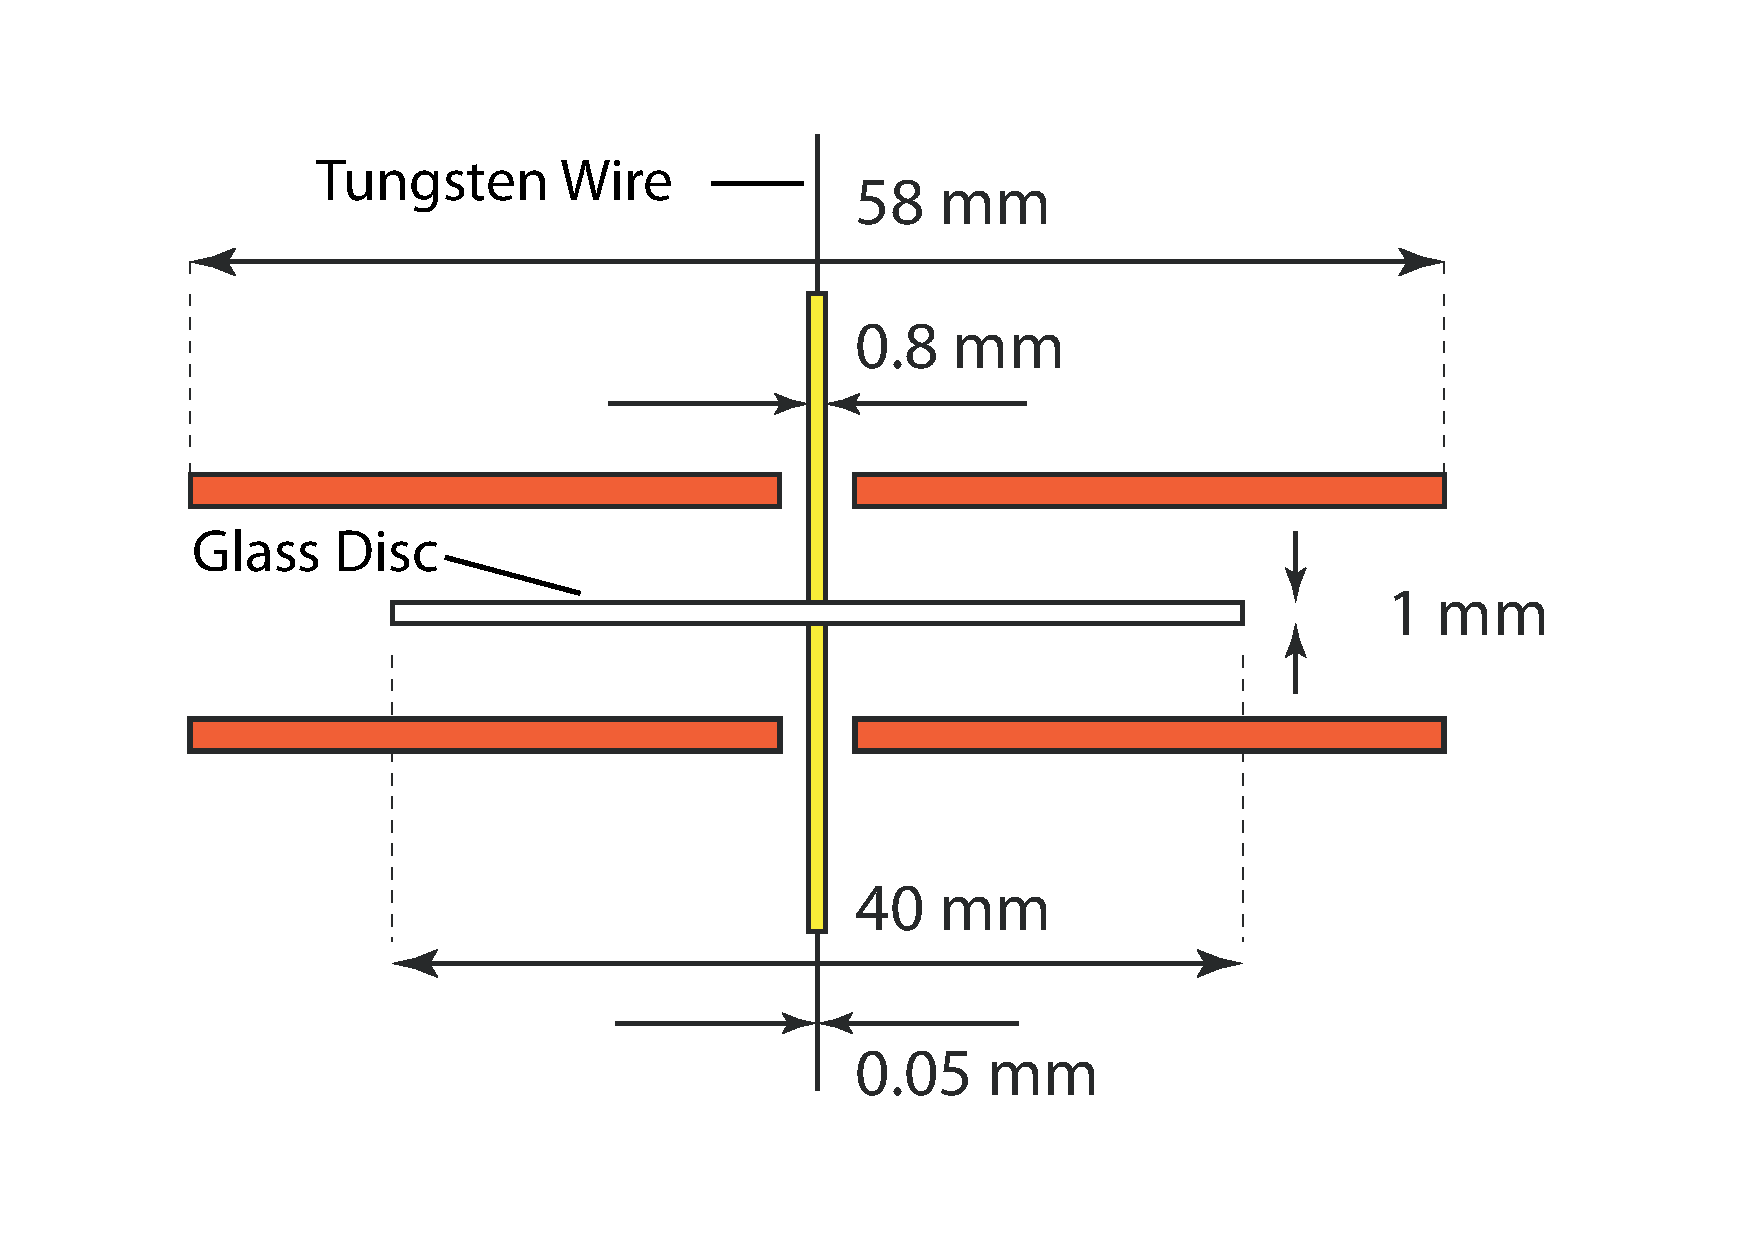
\includegraphics[width=0.7\textwidth]{graphics/exp/disc}
	\caption{Schematic diagram of the torsionally oscilating disc. Source: \cite{universal_scaling}}
	\label{disc}
\end{figure}

The raw data is in the form of video recordings of the disc motion and fairly complex post-processing method was required to extract quantities. The optical distortion from the lenses and the curved walls of the cryostat are negligible.

\newpage
